\documentclass[11pt]{article}
\usepackage[UTF8]{ctex}
\usepackage{subcaption}
%%%%%%%%%%%%%%%%%%%%%%%%%%%%%%%%%%%%%%%%%
% Cleese Assignment
% Structure Specification File
% Version 1.0 (27/5/2018)
%
% This template originates from:
% http://www.LaTeXTemplates.com
%
% Author:
% Vel (vel@LaTeXTemplates.com)
%
% License:
% CC BY-NC-SA 3.0 (http://creativecommons.org/licenses/by-nc-sa/3.0/)
%
%%%%%%%%%%%%%%%%%%%%%%%%%%%%%%%%%%%%%%%%%

%----------------------------------------------------------------------------------------
%	PACKAGES AND OTHER DOCUMENT CONFIGURATIONS
%----------------------------------------------------------------------------------------

\usepackage{lastpage} % Required to determine the last page number for the footer

\usepackage{graphicx} % Required to insert images

\setlength\parindent{0pt} % Removes all indentation from paragraphs

\usepackage[most]{tcolorbox} % Required for boxes that split across pages

\usepackage{booktabs} % Required for better horizontal rules in tables

\usepackage{listings} % Required for insertion of code

\usepackage{etoolbox} % Required for if statements

\usepackage{amsmath}
\usepackage{amsthm}
\usepackage{amssymb}
\usepackage{indentfirst}
\usepackage{diagbox}
\usepackage{subfigure}
\usepackage{float}
\usepackage{xcolor}
\usepackage[colorlinks, linkcolor = black]{hyperref}

\usepackage{enumerate}
\usepackage{enumitem}
\setlist{
    leftmargin = .1\linewidth,
    % rightmargin = .1\linewidth,
    % label=\emph{\alph*}.
}

\setlength{\parindent}{2em}

\usepackage{siunitx}
\sisetup
{
    output-exponent-marker = \ensuremath{\mathrm{E}},
    exponent-product = {},
    retain-explicit-plus,
    retain-zero-exponent,
}
%----------------------------------------------------------------------------------------
%	MARGINS
%----------------------------------------------------------------------------------------

\usepackage{geometry} % Required for adjusting page dimensions and margins

\geometry{
    paper=a4paper, % Change to letterpaper for US letter
    top=3cm, % Top margin
    bottom=3cm, % Bottom margin
    left=2.5cm, % Left margin
    right=2.5cm, % Right margin
    headheight=14pt, % Header height
    footskip=1.4cm, % Space from the bottom margin to the baseline of the footer
    headsep=1.2cm, % Space from the top margin to the baseline of the header
    %showframe, % Uncomment to show how the type block is set on the page
}

%----------------------------------------------------------------------------------------
%	FONT
%----------------------------------------------------------------------------------------

\usepackage[utf8]{inputenc} % Required for inputting international characters
\usepackage[T1]{fontenc} % Output font encoding for international characters

% \usepackage[sfdefault,light]{roboto} % Use the Roboto font

%----------------------------------------------------------------------------------------
%	HEADERS AND FOOTERS
%----------------------------------------------------------------------------------------

\usepackage{fancyhdr} % Required for customising headers and footers

\pagestyle{fancy} % Enable custom headers and footers

\lhead{\small\assignmentClass} % Left header; output the instructor in brackets if one was set
\chead{\small\assignmentTitle} % Centre header
\rhead{\small\ifdef{\assignmentAuthorName}{\assignmentAuthorName}{\ifdef{\assignmentDate}{Due\ \assignmentDate}{}}} % Right header; output the author name if one was set, otherwise the due date if that was set

\lfoot{} % Left footer
\cfoot{\small Page\ \thepage\ of\ \pageref{LastPage}} % Centre footer
\rfoot{} % Right footer

\renewcommand\headrulewidth{0.5pt} % Thickness of the header rule

%----------------------------------------------------------------------------------------
%	MODIFY SECTION STYLES
%----------------------------------------------------------------------------------------

\usepackage{titlesec} % Required for modifying sections

%------------------------------------------------
% Section

\titleformat
{\section} % Section type being modified
[block] % Shape type, can be: hang, block, display, runin, leftmargin, rightmargin, drop, wrap, frame
{\Large\bfseries} % Format of the whole section
{\arabic{section}} % Format of the section label
{6pt} % Space between the title and label
{} % Code before the label

\titlespacing{\section}{0pt}{0.5\baselineskip}{0.5\baselineskip} % Spacing around section titles, the order is: left, before and after

%------------------------------------------------
% Subsection

\titleformat
{\subsection} % Section type being modified
[block] % Shape type, can be: hang, block, display, runin, leftmargin, rightmargin, drop, wrap, frame
{\itshape} % Format of the whole section
{(\arabic{subsection})} % Format of the section label
{4pt} % Space between the title and label
{} % Code before the label

\titlespacing{\subsection}{0pt}{0.5\baselineskip}{0.5\baselineskip} % Spacing around section titles, the order is: left, before and after

\renewcommand\thesubsection{(\arabic{subsection})}

%----------------------------------------------------------------------------------------
%	CUSTOM QUESTION COMMANDS/ENVIRONMENTS
%----------------------------------------------------------------------------------------



% Command to print an assignment section title to split an assignment into major parts
\newcommand{\assignmentSection}[1]{
    \newpage
    {
        \centering % Centre the section title
        \vspace{2\baselineskip} % Whitespace before the entire section title

        \rule{0.8\textwidth}{0.5pt} % Horizontal rule

        \vspace{0.75\baselineskip} % Whitespace before the section title
        {\LARGE \textsc{#1}} % Section title, forced to be uppercase

        \rule{0.8\textwidth}{0.5pt} % Horizontal rule

        \vspace{\baselineskip} % Whitespace after the entire section title
    }
    \setcounter{section}{0}

}

%----------------------------------------------------------------------------------------
%	TITLE PAGE
%----------------------------------------------------------------------------------------

\author{\textbf{\assignmentNo\ \assignmentAuthorName}} % Set the default title page author field
\date{} % Don't use the default title page date field

\title{
    \thispagestyle{empty} % Suppress headers and footers
    \vspace{0.2\textheight} % Whitespace before the title
    \textbf{\assignmentClass}\\[5pt]
    \texttt{\assignmentTitle}\\[-4pt]
    % \ifdef{\assignmentSubTitle}{\texttt{\assignmentSubTitle}}{}
    \ifdef{\assignmentDate}{\assignmentDate}{} % If a due date is supplied, output it
    \ifdef{\assignmentClassInstructor}{{\large \textit{\assignmentClassInstructor}}}{} % If an instructor is supplied, output it
    \vspace{0.32\textheight} % Whitespace before the author name
}


\sisetup
{
    table-format = +1.12e+003,
}

\newcommand{\assignmentQuestionName}{Question} % The word to be used as a prefix to question numbers; example alternatives: Problem, Exercise
\newcommand{\assignmentClass}{计算方法B} % Course/class
\newcommand{\assignmentTitle}{Programming Assignment\ \#4}
\newcommand{\assignmentDate}{2020.5.10} % date
\newcommand{\assignmentNo}{PB17000297}
\newcommand{\assignmentAuthorName}{罗晏宸} % Student name

\begin{document}

\maketitle % Print the title page

\thispagestyle{empty} % Suppress headers and footers on the title page

\newpage

\assignmentSection{迭代法解线性代数方程组}
\section{问题描述}
分别编写Jacobi迭代及Gauss-Seidel迭代的通用程序,注意,不容许对矩阵作求逆运算。分别用如上程序求下述方程组的解,请输出各自的迭代步数以及数值解。

考虑线性代数方程组 $Ax = b$,其中
\begin{align*}
    A & =
    \begin{pmatrix}
        \phantom{-}2 & -1           &        &              &              \\
        -1           & \phantom{-}2 & -1     &              &              \\
                     & \ddots       & \ddots & \ddots       &              \\
                     &              & -1     & \phantom{-}2 & -1           \\
                     &              &        & -1           & \phantom{-}2
    \end{pmatrix}_{10 \times 10}
    \text{为三角矩阵}                                       \\
    b & = (2,\, \cdots,\, 2)^\mathbf{T} \in \mathbb{R}^{10}
\end{align*}

取初始迭代 $x^{(0)} = (0, 0, \cdots, 0)^\mathbf{T}$、停止条件 $\left\Arrowvert x^{(k + 1)} - x^{(k)} \right\Arrowvert_{\infty} \leqslant 10^{-5}$,请输出各自的迭代次数以及最终的数值解。通过本次实验,讨论并比较两种迭代方法的优缺点(比如收敛速度等等),给出实验小结。

\section{计算结果}

由 C++ 通过两种迭代方式计算得到数值解如表所示,
\begin{figure}[h]
    \centering
    \begin{subfigure}{.49\textwidth}
        \centering
        \begin{tabular}{|c|c|}
            \hline $x^{(k)}_1$    & $9.9999301572\text{E}{+}000$ \\
            \hline $x^{(k)}_2$    & $1.7999865973\text{E}{+}001$ \\
            \hline $x^{(k)}_3$    & $2.3999812646\text{E}{+}001$ \\
            \hline $x^{(k)}_4$    & $2.7999774498\text{E}{+}001$ \\
            \hline $x^{(k)}_5$    & $2.9999754619\text{E}{+}001$ \\
            \hline $x^{(k)}_6$    & $2.9999754619\text{E}{+}001$ \\
            \hline $x^{(k)}_7$    & $2.7999774498\text{E}{+}001$ \\
            \hline $x^{(k)}_8$    & $2.3999812646\text{E}{+}001$ \\
            \hline $x^{(k)}_9$    & $1.7999865973\text{E}{+}001$ \\
            \hline $x^{(k)}_{10}$ & $9.9999301572\text{E}{+}000$ \\
            \hline
        \end{tabular}
        \caption{Jacobi 迭代数值解}
    \end{subfigure}
    \begin{subfigure}{.49\textwidth}
        \centering
        \begin{tabular}{|c|c|}
            \hline $x^{(k)}_1$    & $9.9999590139\text{E}{+}000$ \\
            \hline $x^{(k)}_2$    & $1.7999924534\text{E}{+}001$ \\
            \hline $x^{(k)}_3$    & $2.3999898781\text{E}{+}001$ \\
            \hline $x^{(k)}_4$    & $2.7999883107\text{E}{+}001$ \\
            \hline $x^{(k)}_5$    & $2.9999877954\text{E}{+}001$ \\
            \hline $x^{(k)}_6$    & $2.9999882898\text{E}{+}001$ \\
            \hline $x^{(k)}_7$    & $2.7999896744\text{E}{+}001$ \\
            \hline $x^{(k)}_8$    & $2.3999917687\text{E}{+}001$ \\
            \hline $x^{(k)}_9$    & $1.7999943501\text{E}{+}001$ \\
            \hline $x^{(k)}_{10}$ & $9.9999717504\text{E}{+}000$ \\
            \hline
        \end{tabular}
        \caption{Gauss-Seidel 迭代数值解}
    \end{subfigure}
\end{figure}
其中 Jacobi 迭代次数为 284 次,Gauss-Seidel 迭代次数为 151 次。

\section{结果分析}
使用 Mathematica 计算得到线性方程组的准确解为
\begin{equation*}
    x^* =    ( 10, 18, 24, 28, 30, 30, 28, 24, 18, 10 ) ^ \mathbf{T}
\end{equation*}
观察得使用迭代算法得到的数值解和准确解在各个分量上的误差均不超过$10^{-4}$,计算可得 Jacob1 迭代所得数值解误差
\begin{equation*}
    e_1 = \left\Arrowvert x^{(k)} - x^{*} \right\Arrowvert_{\infty} = \max_{i}{|x^{(k)}_i - x^{*}_i|} = 0.000245381
\end{equation*}
Gauss-Seidel 迭代所得数值解误差
\begin{equation*}
    e_2 = \left\Arrowvert x^{(k)} - x^{*} \right\Arrowvert_{\infty} = \max_{i}{|x^{(k)}_i - x^{*}_i|} = 0.000122046
\end{equation*}
这表明两组计算实际上均向准确值收敛,设置停止条件也有效控制了误差,对比之下,Gauss-Seidel 迭代的误差控制的更好。并且在相同的计算误差停止条件控制下,Gauss-Seidel 法迭代次数显著少于 Jacobi 法迭代,迭代速度较快。为进一步观察两组方法的迭代效果,使用 Mathematica 按色相填充迭代过程中的每个向量,每一次迭代的结果对应图中的一列方格,颜色的冷暖对应分量数值的大小,如图\ref{figure:1}所示,
\begin{figure}[h]
    \centering
    \begin{subfigure}{\textwidth}
        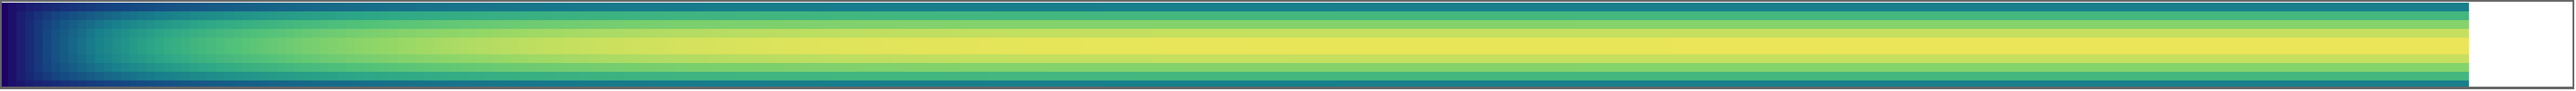
\includegraphics[scale = 0.32]{Figure/Jacobi_284.pdf}
        \caption{Jacobi}
        \label{figure:Jacobi-1}
    \end{subfigure}
    \begin{subfigure}{\textwidth}
        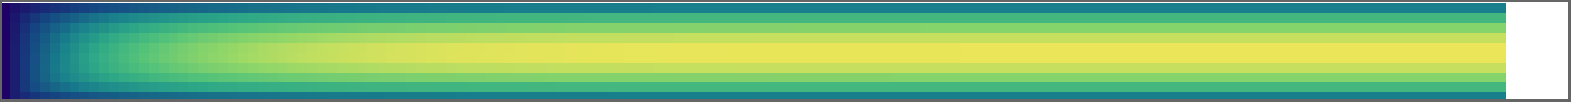
\includegraphics[scale = 0.32]{Figure/Gauss_Seidel_151.pdf}
        \caption{Gauss-Seidel}
        \label{figure:Gauss-Seidel-1}
    \end{subfigure}
    \caption{迭代过程色相图}
    \label{figure:1}
\end{figure}
除了因迭代次数不同两幅色相图的宽度不同外,注意到迭代开始时两者颜色变化速度有着一定差异,为进一步观察,截取两幅色相图左侧 60 格宽度的部分进行对比
\begin{figure}[h]
    \centering
    \begin{subfigure}{\textwidth}
        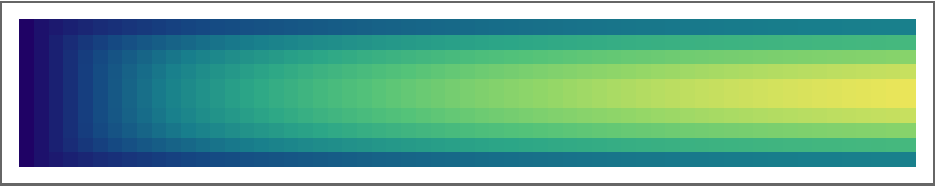
\includegraphics{Figure/Jacobi_60.pdf}
        \caption{Jacobi 迭代过程色相图前 60 格}
        \label{figure:Jacobi-2}
        \label{}
    \end{subfigure}
    \begin{subfigure}{\textwidth}
        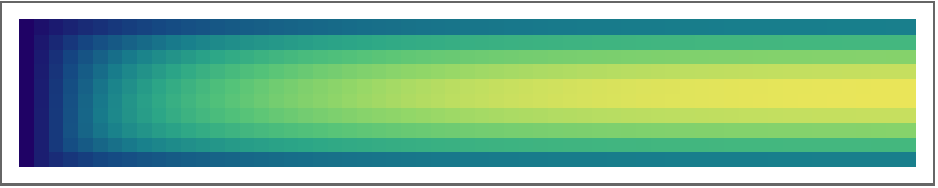
\includegraphics{Figure/Gauss_Seidel_60.pdf}
        \caption{Gauss-Seidel 迭代过程色相图前 60 格}
        \label{figure:Gauss-Seidel-2}
        \label{}
    \end{subfigure}
    \caption{迭代过程色相图(部分)}
    \label{figure:2}
\end{figure}
可以较为清晰地注意到,Jacobi 迭代对应色相图开始部分的中部(对应$x^{(k)}_5$附近的分量)有一定长度的绿色(数值较小),而 Gauss-Seidel 迭代则很快变为黄色(数值较大),结合此方程的实际解的数值特征(分量$x^{(k)}_5$、$x^{(k)}_6$最大,分量$x^{(k)}_1$、$x^{(k)}_{10}$最小),这表明相比 Jacobi 迭代,Gauss-Seidel 迭代能够更为快速地收敛到解附近。

\section{算法分析}
通过对计算结果的分析可知,Gauss-Seidel 迭代在误差控制和收敛速度上均优于 Jacobi 迭代。两者在算法上的主要差异为,Gauss-Seidel 迭代及时使用了更新后的向量分量,从而提升了大部分情况下的算法表现与收敛效果。

另外注意到,计算中使用的停止条件约束了每次迭代前后的向量之差,在计算中包含一定更新信息的 Gauss-Seidel 算法并没有在迭代后期因迭代前后向量差异较小而过早终止,而是将误差控制在一个更好的范围内(相比 Jacobi 迭代)。

\section{实验结论}
本次实验通过对同一个线性方程组在同一初始及停止条件下使用两种不同的迭代方法进行数值求解,对比了 Jacobi 迭代和 Gauss-Seidel 迭代各自的迭代速度、误差控制。在通常情况下,如果两种迭代均收敛,那么后者有着更好的收敛效果。


\end{document}






